\documentclass[11pt,a4paper]{report}

% ---------- Packages ----------
\usepackage[a4paper,margin=2.5cm]{geometry}
\usepackage[utf8]{inputenc}
\usepackage[T1]{fontenc}
\usepackage{titlesec}
\usepackage{fancyhdr}
\usepackage{graphicx}
\usepackage{xcolor}
\usepackage{booktabs}
\usepackage{longtable}
\usepackage{array}
\usepackage{tabularx}
\usepackage{enumitem}
\usepackage{amsmath}
\usepackage{amssymb}
\usepackage{tikz}
\usetikzlibrary{shapes.geometric,arrows.meta,positioning,fit,backgrounds,calc,decorations.pathreplacing}
\usepackage{hyperref}
\usepackage{caption}
\usepackage{float}
\usepackage{parskip}
\usepackage{tcolorbox}
\tcbuselibrary{skins,breakable}

% ---------- Colours ----------
\definecolor{navy}{RGB}{20,40,90}
\definecolor{steel}{RGB}{70,110,160}
\definecolor{lightblue}{RGB}{223,235,246}
\definecolor{mint}{RGB}{213,240,226}
\definecolor{peach}{RGB}{253,232,214}
\definecolor{rose}{RGB}{250,220,220}
\definecolor{grayline}{RGB}{90,90,90}
\definecolor{codebg}{RGB}{244,244,244}

% ---------- Section styling ----------
\titleformat{\chapter}[display]
  {\normalfont\bfseries\color{navy}}
  {\Large\chaptertitlename\ \thechapter}
  {6pt}{\Huge}
\titleformat{\section}
  {\normalfont\Large\bfseries\color{navy}}{\thesection}{0.6em}{}
\titleformat{\subsection}
  {\normalfont\large\bfseries\color{steel}}{\thesubsection}{0.6em}{}
\titleformat{\subsubsection}
  {\normalfont\bfseries\color{steel}}{\thesubsubsection}{0.6em}{}

\pagestyle{fancy}
\fancyhf{}
\renewcommand{\headrulewidth}{0.4pt}
\fancyhead[L]{\small\textit{A Privacy-Preserving Edge Gateway for Audio Deepfake Detection}}
\fancyhead[R]{\small\thepage}
\fancyfoot[C]{\small\textcolor{gray}{Confidential inference project narrative --- prepared for supervisory review}}

\hypersetup{
  colorlinks=true,
  linkcolor=steel,
  citecolor=steel,
  urlcolor=steel,
  pdftitle={A Privacy-Preserving Edge Gateway for Real-Time Audio Deepfake Detection},
  pdfauthor={Waleed Asif}
}

% ---------- Helper boxes ----------
\newtcolorbox{decisionbox}[1]{
  breakable, enhanced, colback=lightblue, colframe=steel,
  boxrule=0.6pt, arc=2pt, left=6pt, right=6pt, top=5pt, bottom=5pt,
  title={\small\bfseries #1}, fonttitle=\color{navy}
}
\newtcolorbox{crisisbox}[1]{
  breakable, enhanced, colback=rose, colframe=red!55!black,
  boxrule=0.6pt, arc=2pt, left=6pt, right=6pt, top=5pt, bottom=5pt,
  title={\small\bfseries #1}, fonttitle=\color{red!55!black}
}
\newtcolorbox{resolvedbox}[1]{
  breakable, enhanced, colback=mint, colframe=green!40!black,
  boxrule=0.6pt, arc=2pt, left=6pt, right=6pt, top=5pt, bottom=5pt,
  title={\small\bfseries #1}, fonttitle=\color{green!30!black}
}
\newtcolorbox{findingbox}[1]{
  breakable, enhanced, colback=peach, colframe=orange!70!black,
  boxrule=0.6pt, arc=2pt, left=6pt, right=6pt, top=5pt, bottom=5pt,
  title={\small\bfseries #1}, fonttitle=\color{orange!60!black}
}

\newcommand{\code}[1]{\texttt{\small #1}}

% Reduce overfull boxes from long unbreakable code tokens
\setlength{\emergencystretch}{2.5em}
\sloppy

% TikZ node styles used across several diagrams
\tikzset{
  block/.style = {rectangle, rounded corners, draw=steel, very thick,
    fill=lightblue, text width=4.6cm, align=center, minimum height=1.05cm, font=\small},
  smallblock/.style = {rectangle, rounded corners, draw=steel, thick,
    fill=lightblue, text width=3.4cm, align=center, minimum height=0.9cm, font=\scriptsize},
  greenblock/.style = {rectangle, rounded corners, draw=green!40!black, very thick,
    fill=mint, text width=4.6cm, align=center, minimum height=1.05cm, font=\small},
  redblock/.style = {rectangle, rounded corners, draw=red!55!black, very thick,
    fill=rose, text width=4.6cm, align=center, minimum height=1.05cm, font=\small},
  orangeblock/.style = {rectangle, rounded corners, draw=orange!70!black, very thick,
    fill=peach, text width=4.6cm, align=center, minimum height=1.05cm, font=\small},
  decblock/.style = {diamond, draw=steel, very thick, fill=lightblue, aspect=2.4,
    text width=3.6cm, align=center, font=\scriptsize, inner sep=2pt},
  arrow/.style = {-{Stealth[length=2.5mm]}, thick, draw=grayline},
  worldbox/.style = {rectangle, draw=grayline, dashed, thick, inner sep=10pt, rounded corners}
}

\begin{document}

% ===================================================================
\begin{titlepage}
\centering
\vspace*{1.2cm}
{\large Atlantic Technological University Galway\par}
{\large Department of Computer Science and Applied Physics\par}
\vspace{1.6cm}
{\color{navy}\Huge\bfseries A Privacy-Preserving Edge Gateway\par}
\vspace{0.3cm}
{\color{navy}\Huge\bfseries for Real-Time Audio Deepfake Detection\par}
\vspace{0.8cm}
{\LARGE Confidential Inference on ARM TrustZone: \par}
{\LARGE the Full Project Journey\par}
\vspace{1.6cm}
{\large\itshape A narrative account of the design decisions, alternatives, risks,\\
and points of difficulty encountered while building and validating\\
the confidential-inference component of the thesis\par}
\vspace{2.2cm}

\begin{tabular}{rl}
\textbf{Author:} & Waleed Asif \\[3pt]
\textbf{Programme:} & MSc Computing \\[3pt]
\textbf{Supervisor:} & Dr.\ Owen Foley \\[3pt]
\textbf{Institution:} & Atlantic Technological University Galway \\[3pt]
\textbf{Document date:} & September 2026 \\
\end{tabular}

\vfill
{\small\itshape Prepared for supervisory review --- this document tells the complete story of the\\
confidential-inference proof-of-concept: what was built, why each method was chosen over\\
the alternatives, where the work got stuck, and how each obstacle was resolved.\par}
\vspace{0.5cm}
\end{titlepage}

\tableofcontents
\clearpage

% ===================================================================
\chapter{Introduction}

\section{What this document is}

This document is a narrative account, not a formal thesis chapter. Its purpose is to walk
through the confidential-inference proof-of-concept (PoC) from the beginning: what problem it
solves, why each significant design decision was made the way it was, which alternatives were
considered and rejected, and --- most importantly for a supervisory review --- exactly where the
project got stuck, what the failure looked like, and how it was diagnosed and resolved. Numeric
results, verification evidence, and known limitations are reported honestly, including one
negative research finding that turned out to be a legitimate contribution in its own right rather
than a bug to hide.

The account is organised chronologically, in the order the work actually happened, because the
reasoning behind later decisions frequently depends on what was learned at an earlier stage.

\section{The thesis in one paragraph}

The overall thesis proposes a privacy-preserving edge gateway for real-time audio deepfake
detection in residential telephony: a small device sitting between a phone line and the call
itself, listening for synthetic-speech characteristics while the call is in progress, and doing so
without exposing the caller's voice or the detection model to whatever else is running on that
device. The detection backbone is a pretrained lightweight neural network, RawTFNet-16
(checkpoint \code{Best\_RawTFNet\_16.pth}). The confidentiality property is provided by ARM
TrustZone, via the open-source OP-TEE trusted execution environment. The intended deployment
target is a Raspberry Pi 4. No physical Pi 4 was available during this phase of the work, so the
entire proof-of-concept described here was built and verified on an emulated ARMv8-A platform
instead --- a substitution that is itself one of the first design decisions this document
justifies.

\section{Why confidential inference, specifically}

A plain spoof-detection classifier running as an ordinary process is not enough for the threat
model this thesis targets. Two properties distinguish the intended system from a bare classifier:

\begin{itemize}[leftmargin=1.4em]
  \item \textbf{Live, not post-hoc, detection.} A decision has to be available while the call is
  still connected, using a rolling audio buffer, rather than analysing a recording after the call
  has ended.
  \item \textbf{Confidential inference.} The input is a person's voice and the model represents
  proprietary work; the inference computation itself should be shielded from a compromised or
  malicious host operating system. This is what ARM TrustZone provides: a hardware-enforced
  isolated execution mode where code and memory can be marked secure-world-only, so that even a
  fully compromised normal-world OS --- kernel included --- cannot read or tamper with what runs
  inside it.
\end{itemize}

No existing peer-reviewed work combines federated learning, differential privacy, and
TrustZone-based confidential inference specifically for anti-spoofing (see Chapter~\ref{sec:rq}).
This proof-of-concept is the first concrete step toward closing that gap for the thesis: it
establishes that the confidential-inference half of that combination is achievable, before the
federated-learning and differential-privacy halves are layered on top in later work.

\chapter{Background}

\section{The detection backbone: RawTFNet-16}
\label{sec:rawtfnet}

RawTFNet (Xiao, Dang and Das, \textit{RawTFNet: A Lightweight CNN Architecture for Speech
Anti-spoofing}, APSIPA ASC 2025) is a lightweight, end-to-end anti-spoofing network. It takes the
raw audio waveform directly as input --- there is no hand-crafted front end, no MFCCs, no
spectrogram, no CQT. All feature extraction happens inside the network's own learnable Sinc layer.
Each utterance is cropped or zero-padded to a fixed-length segment of approximately four seconds
(64,600 samples at 16\,kHz in this project's checkpoint), and that fixed length is structural: it
cannot be shortened without the network's internal pooling operations collapsing to zero size (a
failure encountered directly and discussed in Section~\ref{sec:window-attempt}).

\begin{figure}[H]
\centering
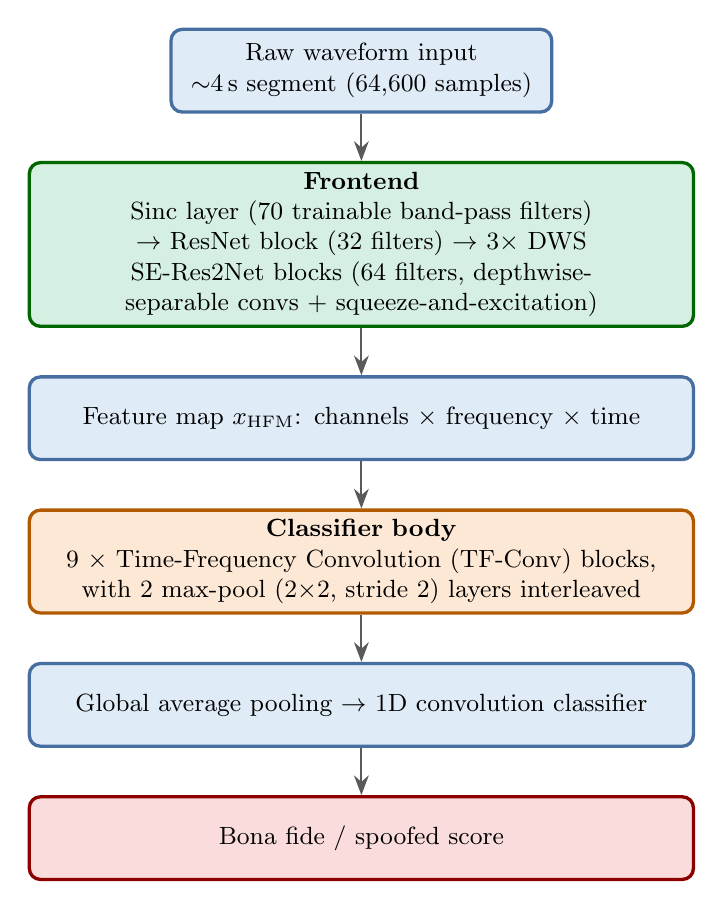
\begin{tikzpicture}[node distance=6mm]
\node[block] (input) {Raw waveform input\\ $\sim$4\,s segment (64{,}600 samples)};
\node[greenblock, below=of input, text width=8.2cm] (frontend)
  {\textbf{Frontend}\\ Sinc layer (70 trainable band-pass filters) $\rightarrow$ ResNet block
  (32 filters) $\rightarrow$ 3$\times$ DWS SE-Res2Net blocks (64 filters, depthwise-separable
  convs + squeeze-and-excitation)};
\node[block, below=of frontend, text width=8.2cm] (feat) {Feature map $x_{\mathrm{HFM}}$: channels
  $\times$ frequency $\times$ time};
\node[orangeblock, below=of feat, text width=8.2cm] (tfconv) {\textbf{Classifier body}\\ 9
  $\times$ Time-Frequency Convolution (TF-Conv) blocks, with 2 max-pool (2$\times$2, stride 2)
  layers interleaved};
\node[block, below=of tfconv, text width=8.2cm] (gap) {Global average pooling $\rightarrow$ 1D
  convolution classifier};
\node[redblock, below=of gap, text width=8.2cm] (out) {Bona fide / spoofed score};
\draw[arrow] (input) -- (frontend);
\draw[arrow] (frontend) -- (feat);
\draw[arrow] (feat) -- (tfconv);
\draw[arrow] (tfconv) -- (gap);
\draw[arrow] (gap) -- (out);
\end{tikzpicture}
\caption{RawTFNet-16 architecture as trained and used unmodified as the detection backbone.
Channel-width parameter $\tau=16$: 0.07M parameters, 2.9G multiply--accumulate operations (MACs)
per 4-second window. The green/orange split marks exactly where this project later cut the network
in two --- see Section~\ref{sec:partition}.}
\label{fig:rawtfnet-arch}
\end{figure}

Table~\ref{tab:rawtfnet-compare} places RawTFNet-16 against the other anti-spoofing systems it was
benchmarked against in the source paper. It is the smallest model in the comparison --- an order of
magnitude fewer parameters than RawNet2 --- while reaching the lowest equal error rate (EER) on the
ASVspoof 2021 LA evaluation set. That combination of footprint and accuracy is what makes it a
realistic choice for confidential inference inside a memory-constrained TrustZone enclave, and is
why it was selected as this project's detection backbone rather than a larger architecture such as
AASIST or RawNet2.

\begin{table}[H]
\centering
\small
\begin{tabular}{lrrrr}
\toprule
Model & Params & MACs & 2021 LA EER & 2021 DF EER \\
\midrule
RawNet2       & 17.60M & 0.8G & 9.50\%  & 22.38\% \\
AASIST        & 0.30M  & 8.9G & 10.51\% & 21.07\% \\
SE-Rawformer  & 0.37M  & 6.1G & 4.98\%  & 20.26\% \\
\textbf{RawTFNet-16} & \textbf{0.07M} & \textbf{2.9G} & \textbf{4.50\%} & 18.53\% \\
RawTFNet-32   & 0.17M  & 5.4G & 5.05\%  & \textbf{16.82\%} \\
\bottomrule
\end{tabular}
\caption{Single-system comparison on ASVspoof 2021 LA and DF (lower EER is better). Source: Xiao,
Dang and Das, APSIPA ASC 2025.}
\label{tab:rawtfnet-compare}
\end{table}

Two properties of the published model directly shaped later engineering decisions in this project:

\begin{itemize}[leftmargin=1.4em]
  \item \textbf{Duration sensitivity.} EER is worst on very short clips (0--2\,s, over 10\%), best
  around 2--4\,s (matching the training segment length), and rises again for 4--8\,s clips. This is
  why the live-detection design (Section~\ref{sec:asterisk}) uses a 4-second sliding window rather
  than a shorter one, even though a shorter window would reduce latency.
  \item \textbf{Ablations on the TF-Conv design.} Removing the frequency branch raises EER from
  5.05\% to 6.91\%; removing the time branch raises it to 7.08\%; removing the channel shuffle
  raises it to 5.74\% at no change in model size. Both branches contribute meaningfully, which is
  one more reason the architecture was used exactly as published rather than simplified for
  easier embedding.
\end{itemize}

No changes were made to the network topology, layer widths, or channel-width parameter
$\tau=16$ anywhere in this project. Every adaptation described in this document is in \emph{how
the already-trained model is deployed} --- exporting it, compiling it, and running it inside a
trusted application --- never in the network itself.

\section{ARM TrustZone and OP-TEE}
\label{sec:trustzone}

ARM TrustZone splits a single physical CPU into two isolated execution states: a \textit{normal
world} and a \textit{secure world}, enforced in hardware rather than by the operating system. Code,
memory, and peripherals can be marked secure-world-only, so that even a fully compromised
normal-world operating system --- kernel included --- cannot read or tamper with what runs in the
secure world.

OP-TEE is the open-source trusted OS that runs inside the secure world and exposes this split
through a standard programming model with two halves:

\begin{itemize}[leftmargin=1.4em]
  \item \textbf{Trusted Application (TA)} --- code that executes inside the secure world. TAs are
  written in C, compiled against OP-TEE's TA development kit, cryptographically signed, and loaded
  on demand into a minimal, single-threaded environment with a small, fixed secure-memory heap.
  \item \textbf{Client Application (CA)} --- an ordinary Linux program in the normal world. A CA
  opens a session with a TA and invokes commands through the GlobalPlatform TEE Client API
  (\code{libteec}).
\end{itemize}

\begin{figure}[H]
\centering
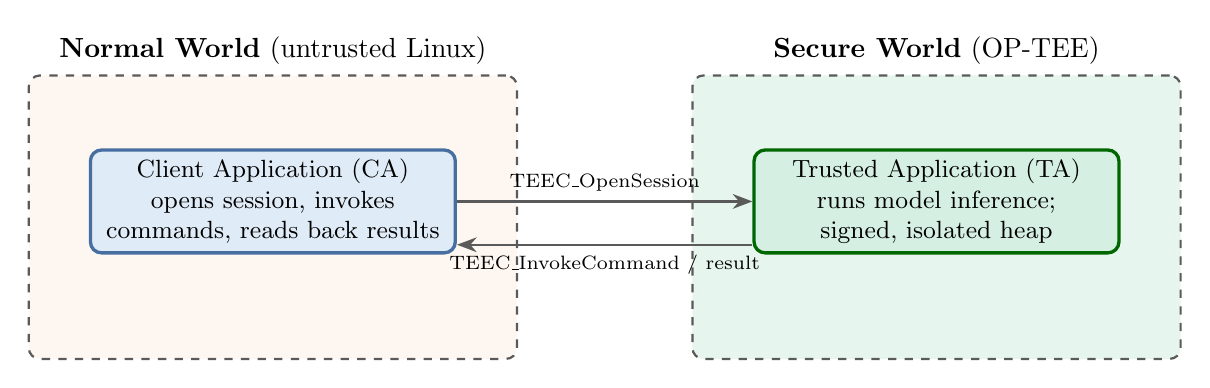
\begin{tikzpicture}[node distance=8mm and 14mm]
\node[worldbox, fill=peach!35, minimum width=6.2cm, minimum height=3.6cm] (nw) {};
\node[above] at (nw.north) {\textbf{Normal World} (untrusted Linux)};
\node[worldbox, fill=mint!60, minimum width=6.2cm, minimum height=3.6cm, right=22mm of nw] (sw) {};
\node[above] at (sw.north) {\textbf{Secure World} (OP-TEE)};

\node[block, minimum width=4.4cm, text width=4.4cm] at ($(nw)+(0,0.2)$) (ca)
  {Client Application (CA)\\ opens session, invokes commands, reads back results};
\node[greenblock, minimum width=4.4cm, text width=4.4cm] at ($(sw)+(0,0.2)$) (ta)
  {Trusted Application (TA)\\ runs model inference; signed, isolated heap};

\draw[arrow] (ca.east) -- node[above, font=\scriptsize] {TEEC\_OpenSession} (ta.west);
\draw[arrow] ($(ta.west)+(0,-0.55)$) -- node[below, font=\scriptsize] {TEEC\_InvokeCommand /
result} ($(ca.east)+(0,-0.55)$);
\end{tikzpicture}
\caption{The TA/CA session pattern: open a session, invoke a command, read back a result. This is
the exact mechanism that carries an audio window into the secure world and a spoof score back out.
It was validated end-to-end using the official \code{hello\_world} example before any
model-specific code was written (Section~\ref{sec:m2}).}
\label{fig:trustzone-split}
\end{figure}

\chapter{Design Decisions and Alternatives Considered}
\label{ch:decisions}

Every major decision in this project was a choice between at least two realistic options. This
chapter records each decision, the alternative that was rejected, and the reasoning --- so that a
reader can see \emph{why} the project looks the way it does, not just what it looks like.

\section{Emulation platform: QEMU ARMv8 ``virt'', not a Raspberry Pi 4 emulator}
\label{sec:qemu-vs-pi4}

\begin{decisionbox}{Decision}
Use the QEMU ``virt'' Armv8-A reference board (the \code{qemu\_v8} manifest in OP-TEE's own build
tooling) as a stand-in for the Raspberry Pi 4, rather than looking for a Pi-4-specific emulator.
\end{decisionbox}

The original plan referred loosely to a ``Raspberry Pi emulator''. This needed to be made precise
before any build work started, and the precise answer is less convenient than the phrase suggests:
\textbf{there is no mainstream, officially maintained emulator that boots a Raspberry Pi 4 with
working TrustZone/OP-TEE support.} Broadcom has never published the secure-boot and TrustZone
configuration details for the BCM2711 SoC used in the Pi 4, so OP-TEE has no official port to that
board, physical or emulated.

The platform actually used instead is a generic ARMv8-A machine with a proper TrustZone-capable
CPU model and full, officially maintained OP-TEE support. This is the standard substitute used
throughout the OP-TEE research and tooling ecosystem, and it shares the same CPU architecture
family (ARMv8-A / AArch64) and the same secure/normal-world security model as the Pi 4's
Cortex-A72. The target deployment platform remains the Raspberry Pi 4; QEMU is used to demonstrate
the feasibility of the confidential-inference \emph{design}, not to reproduce Pi 4
\emph{performance}.

\begin{findingbox}{Honest cost of this substitution}
QEMU/OP-TEE is a \textbf{functional} proxy, not a \textbf{performance} proxy. Two compounding
factors make QEMU timings unrepresentative of a real Pi 4: (1)~the \code{virt} platform does not
model the Pi 4's actual Cortex-A72 cores, cache hierarchy, or memory bandwidth; and (2)~because the
OP-TEE build runs inside an x86\_64 VirtualBox VM, QEMU performs full software instruction
translation (TCG) from ARM64 to x86\_64 with no KVM acceleration --- and CPU-bound workloads such
as neural-network matrix multiplications are exactly what TCG handles worst. TCG-translated,
CPU-bound workloads are commonly 5--20$\times$ slower than native execution; a real Pi~4 running
natively should be expected to beat the QEMU/TCG setup by roughly one to two orders of magnitude
for RawTFNet-16 inference specifically. This is recorded explicitly so that no latency number
produced on QEMU is ever mistaken for a Pi 4 figure in the final thesis.
\end{findingbox}

\section{Development host: VirtualBox Ubuntu 22.04 LTS, not WSL2}
\label{sec:vm-vs-wsl2}

\begin{decisionbox}{Decision}
Develop inside a VirtualBox virtual machine running Ubuntu 22.04 LTS with a \textbf{bridged}
network adapter, instead of using WSL2 on the same Windows machine.
\end{decisionbox}

OP-TEE's build system (the \code{repo} multi-repository tool, Buildroot, device-tree compilation,
cross-toolchains) requires a native Linux environment and does not build reliably under Windows
compatibility layers such as Git Bash/MINGW64. A Linux environment was therefore required either
way; the choice was between WSL2 and a full VM.

A VM was chosen over WSL2 specifically because a later stage of this work needs to receive live
audio from an Asterisk server, and Asterisk's SIP/RTP traffic needs a stable, directly reachable
network address. WSL2's default NAT layer and internal IP volatility are a known source of
unreliability for real-time media traffic, whereas a VirtualBox VM with a bridged network adapter
gives the Linux environment a stable IP on the same LAN as any calling client --- while still
letting Windows (model training, Python tooling) and Linux (OP-TEE, Asterisk) run side by side
without dual-boot reboots. Ubuntu 22.04 LTS specifically was chosen for its long-term support and
strong compatibility with VoIP frameworks, security libraries, and research tooling, reducing the
risk of dependency conflicts through the rest of the project.

In practice the VM's bridged-network IP address changed across several reboots during the project
(observed values included \code{192.168.1.183}, \code{192.168.1.175}, and \code{192.168.0.11}),
which became a minor recurring friction point --- addressed simply by re-checking \code{ip a} before
each file transfer rather than assuming a fixed address.

\section{Model deployment path: PyTorch $\rightarrow$ ONNX $\rightarrow$ C, not hand-ported C}
\label{sec:onnx-path}

\begin{decisionbox}{Decision}
Export the trained PyTorch model to ONNX, verify it numerically at every stage, and compile the
verified graph directly to standalone C for embedding in a Trusted Application --- rather than
hand-porting RawTFNet's layers to C by hand.
\end{decisionbox}

A Trusted Application executes inside a minimal, single-threaded environment with a restricted C
library and a small, fixed secure-memory heap; it cannot host a full deep-learning framework.
PyTorch, ONNX Runtime, and TensorFlow all assume a POSIX-ish environment with dynamic memory,
threads, and large heaps, none of which exists inside a TA. Two options were considered:

\begin{itemize}[leftmargin=1.4em]
  \item \textbf{Hand-port RawTFNet's layers directly to C.} Rejected as high-effort and high-risk:
  every convolution, the Sinc layer, the squeeze-and-excitation modules, and the batch-norm folding
  would need to be reimplemented and independently verified, with numerous opportunities for silent
  numerical divergence from the trained model.
  \item \textbf{Export to ONNX (a framework-neutral graph representation), then compile it
  ahead-of-time to dependency-free C.} Adopted. Correctness is checked numerically at every
  conversion step against the original PyTorch output, so that any discrepancy is caught at the
  specific stage that introduced it, rather than surfacing later inside the TEE where debugging is
  significantly harder.
\end{itemize}

Within this second path, two different tools were tried for the ONNX-to-C step, and one of them was
abandoned. This is documented in detail in Section~\ref{sec:onnx2c-vs-emx}, because it was a real
dead end that cost real time, not a clean first-try success.

\section{Apache TVM: used for independent verification, not for the deployed code}

Apache TVM (0.25.0.post1) was used at one stage of the pipeline, but strictly as an
\textbf{independent cross-check} of the ONNX graph's correctness --- compiling it with TVM's Relax
API and an LLVM JIT target, and confirming the output matched PyTorch and ONNX Runtime to four
decimal places on a held-out test utterance. TVM was deliberately \emph{not} used to generate the
C code that ships inside the deployed Trusted Application; that role belongs to the tool described
in Section~\ref{sec:onnx2c-vs-emx} (\code{emx-onnx-cgen}). Keeping these two roles separate meant
that a numerical mismatch could always be traced to either the export step or the final C codegen
step, never to an ambiguous mixture of both.

One practical difficulty is worth recording for reproducibility: the installed TVM release
(0.25.0.post1) uses the newer Relax API, which has fully replaced the classical Relay API that most
published TVM tutorials and documentation still assume. Import paths such as \code{tvm.relay} and
\code{tvm.nd} no longer exist; the working incantations
(\code{tvm.relax.frontend.onnx.from\_onnx}, \code{tvm.runtime.tensor}) had to be found empirically
by inspecting the installed package rather than by following an existing guide.

\section{Scope of the proof-of-concept}

The full thesis scope combines RawTFNet, TrustZone confidential inference, and federated learning
with differential privacy. That full scope was deliberately narrowed for this phase of the work to
demonstrating the confidential-inference path alone: export the already-trained model and get it
executing inside the TrustZone/OP-TEE environment, deferring federated learning, weight
re-training, and secure key-provisioning for weights to later work. The model's weights are
compiled directly into the TA binary as a static array for this PoC; this is a known simplification
--- it means the TA would need re-signing on every retrain --- and is recorded explicitly in the
limitations (Chapter~\ref{ch:limitations}).

\chapter{System Architecture}

Figure~\ref{fig:end-to-end} shows the target end-to-end pipeline: from a live call, through a
rolling audio buffer and windowing in the normal world, across the TrustZone boundary into the
secure-world classifier, and back out to a live decision. The colour of each stage reflects how
this document is organised: green stages are the model-correctness work (Chapter~\ref{ch:crisis}
onward covers how they were achieved), and everything to the right of the dashed
confidential-inference boundary is protected from a compromised normal-world host.

\begin{figure}[H]
\centering
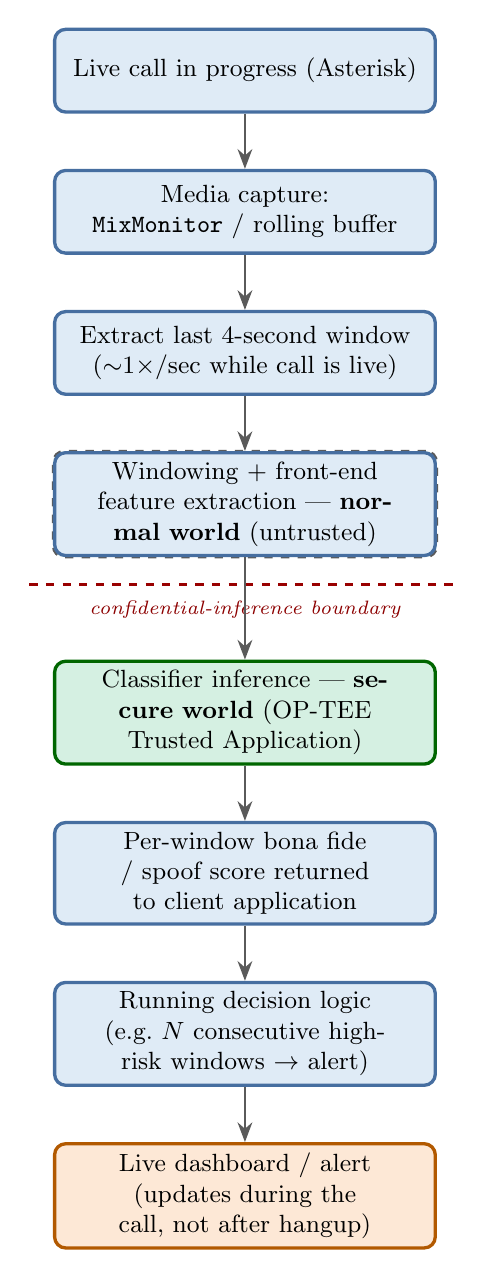
\begin{tikzpicture}[node distance=7mm]
\node[block] (call) {Live call in progress (Asterisk)};
\node[block, below=of call] (capture) {Media capture: \code{MixMonitor} / rolling buffer};
\node[block, below=of capture] (window) {Extract last 4-second window ($\sim$1$\times$/sec while
call is live)};
\node[block, below=of window] (prep) {Windowing + front-end feature extraction --- \textbf{normal
world} (untrusted)};

\begin{scope}[on background layer]
\node[worldbox, fill=mint!45, fit=(prep), inner sep=0pt] {};
\end{scope}

\draw[very thick, dashed, red!60!black] ($(prep.south west)+(-0.3,-0.35)$) --
($(prep.south east)+(0.3,-0.35)$)
  node[midway, below, font=\scriptsize\itshape, text=red!55!black, yshift=-2pt]
  {confidential-inference boundary};

\node[greenblock, below=13mm of prep] (secure) {Classifier inference --- \textbf{secure world}
(OP-TEE Trusted Application)};
\node[block, below=of secure] (score) {Per-window bona fide / spoof score returned to client
application};
\node[block, below=of score] (decision) {Running decision logic (e.g.\ $N$ consecutive high-risk
windows $\rightarrow$ alert)};
\node[orangeblock, below=of decision] (dash) {Live dashboard / alert (updates during the call, not
after hangup)};

\draw[arrow] (call) -- (capture);
\draw[arrow] (capture) -- (window);
\draw[arrow] (window) -- (prep);
\draw[arrow] (prep) -- (secure);
\draw[arrow] (secure) -- (score);
\draw[arrow] (score) -- (decision);
\draw[arrow] (decision) -- (dash);
\end{tikzpicture}
\caption{End-to-end live in-call detection pipeline. Feature extraction (the front-end half of
RawTFNet) currently remains in the untrusted normal world; only the classifier's forward pass
executes inside the secure world for this PoC (Section~\ref{sec:partition} explains why the model
is split at exactly this point). This is a deliberate, stated scope boundary, recorded again in
Chapter~\ref{ch:limitations}.}
\label{fig:end-to-end}
\end{figure}

\chapter{The Implementation Journey}
\label{ch:crisis}

This chapter is the core of the document: a chronological account of every phase of the work,
including the phases that failed on the first attempt, the phases that failed on the \emph{second}
attempt for a different reason, and the one significant misdiagnosis that was caught and corrected
before it could mislead later work.

\section{Phase 1 --- Environment bring-up}

The purpose of this stage was to confirm that the toolchain, cross-compilation, and QEMU boot
process all worked before any project-specific code was written. OP-TEE OS, TF-A, the Linux kernel,
and a Buildroot root filesystem were built for the QEMU Armv8-A \code{virt} platform from the
official manifest, and the environment was booted and the official OP-TEE test suite run against
it.

\begin{resolvedbox}{Result}
System booted with a working secure-world / normal-world split. \code{xtest} completed with
\textbf{0 failures across 41{,}482 subtests and 145 test cases}. This is the standard signal that
the secure/normal-world split is functioning correctly on this platform.
\end{resolvedbox}

Several ordinary build-dependency errors were hit and fixed along the way and are recorded here for
completeness rather than as anything remarkable: \code{libgnutls28-dev} was missing (u-boot's
\code{mkeficapsule} build failed until it was installed); \code{python3-tomli} was missing (the
QEMU meson build failed until it was installed); and one transient HTTP 404 on a QEMU subproject
download resolved itself on retry.

\section{Phase 2 --- Validating the TA/CA communication pattern}
\label{sec:m2}

Before writing any model-specific code, the official \code{hello\_world} TA/CA example was built
and run to validate the exact client-application-to-trusted-application invocation pattern the
model-inference TA would later reuse.

\begin{resolvedbox}{Result}
The client application successfully opened a session with the trusted application and received a
correctly computed result back (the TA incremented a test value from 42 to 43). This de-risks the
communication pattern itself, so that Milestones 4 onward could be scoped as ``plug the verified
model into a known-working pattern'' rather than an open integration risk.
\end{resolvedbox}

\section{Phase 3 --- Exporting and compiling the model}
\label{sec:onnx2c-vs-emx}

\subsection{Export to ONNX and numerical verification}

The trained checkpoint was exported to ONNX with a fixed input shape (no dynamic axes) and all
weights consolidated into a single file rather than external-data references, and its output was
verified against the original PyTorch model on a held-out ASVspoof 2021 LA utterance. Both produced
the same score to four decimal places (PyTorch $-5.6216$, ONNX $-5.6216$; TVM/Relax cross-check
$-5.621588$).

One export-time error surfaced during this stage and is worth recording because it reveals a
structural property of the model, not a tooling bug: attempting to export or run the model on an
input shorter than the native 64,600-sample window fails with
\begin{quote}\small\ttfamily
RuntimeError: Given input size: (24x5x1). Calculated output size: (24x2x0). Output size is too
small
\end{quote}
because the network's internal max-pooling layers collapse a too-short input to zero spatial size.
\label{sec:window-attempt}
This confirmed, independently of the later memory-wall investigation, that the 4-second window is
not an arbitrary convenience but a structural requirement of the trained architecture --- a point
the memory-wall investigation in Section~\ref{sec:memory-wall} returns to directly.

\subsection{The abandoned path: onnx2c}
\label{sec:onnx2c}

\begin{crisisbox}{Dead end}
\code{onnx2c} was the first ONNX-to-C tool tried, and it was abandoned after three consecutive
operator-support gaps made it unusable for this model.
\end{crisisbox}

\code{onnx2c} was cloned and built (using the targeted \code{make onnx2c} build, since the tool's
own full test suite fails on an unrelated \code{\_Float16} target issue that has nothing to do with
this model). Three separate blocking errors were then hit in sequence while trying to compile the
cleaned ONNX graph:

\begin{enumerate}[leftmargin=1.5em]
  \item An external-data tensor reference the tool could not resolve (fixed independently by
  re-exporting ONNX with all weights embedded in one file).
  \item \code{Unknown attribute training\_mode} on \code{BatchNormalization} nodes --- partially
  worked around with \code{onnxsim} simplification and a script that manually stripped the
  attribute, but this treated a symptom rather than a root cause.
  \item \code{No axes to squeeze away?} on a \code{Squeeze} node inside the squeeze-and-excitation
  (SE) module --- this one could not be resolved. The SE module's data-dependent squeeze pattern
  fell outside what \code{onnx2c}'s parser supported, and no workaround was found.
\end{enumerate}

At this point \code{onnx2c} was abandoned for this model, and \code{emx-onnx-cgen} was adopted
instead.

\subsection{The adopted path: emx-onnx-cgen}

\code{emx-onnx-cgen} was chosen over continuing to patch \code{onnx2c} for concrete reasons: it is
pip-installable, reports over 99\% coverage of the ONNX opset-26 operator set, generates static,
malloc-free-by-design\footnote{As Section~\ref{sec:memory-wall} shows, ``malloc-free by design''
described the tool's default posture, not this project's eventual configuration --- the setting
that maximises static allocation (\code{--large-weight-threshold 0}) was exactly the one that later
caused the load failure. This is flagged here and resolved fully in Section~\ref{sec:memory-wall}.}
C, and ships a built-in \code{verify} command that checks the generated C against ONNX Runtime with
explicit ULP (unit-in-the-last-place) tolerance reporting.

The classifier half of the model (the half eventually embedded in the TA; see
Section~\ref{sec:partition}) compiled cleanly and its \code{verify} command reported a maximum
deviation of \textbf{7 ULP} against ONNX Runtime --- an essentially exact match, several orders of
magnitude tighter than would be needed to change a bona-fide/spoof decision.

\section{Phase 4 --- The memory wall}
\label{sec:memory-wall}

This is the most significant obstacle encountered in the entire confidential-inference PoC, and the
one that took the longest to correctly diagnose. It is presented here as a full investigation
narrative, in the order the reasoning actually unfolded, including the theories that turned out to
be wrong.

\subsection{The failure}

With the full model (front-end and classifier together) compiled to a single C file and linked into
a Trusted Application, the very first attempt to open a session against it failed. The client
application reported

\begin{quote}\small\ttfamily
TEEC\_OpenSession failed 0xffff000c
\end{quote}

and the secure-world log showed the load itself failing before the TA ever ran a single instruction:

\begin{quote}\small\ttfamily
E/LD:\ \ populate\_segments:891 sys\_map\_zi\\
E/TC:? 1 ldelf\_init\_with\_ldelf:152 ldelf failed with res: 0xffff000c\\
D/TC:? 1 tee\_ta\_open\_session:722 init session failed 0xffff000c
\end{quote}

\code{sys\_map\_zi} is the loader step that maps a TA's zero-initialised memory (its \code{.bss}
segment and heap reservation) into the secure world before execution starts. A failure here means
the TA's declared memory footprint could not be satisfied by the loader --- not a bug in the model's
logic, but a resource ceiling.

\subsection{Investigation timeline}

\begin{figure}[H]
\centering
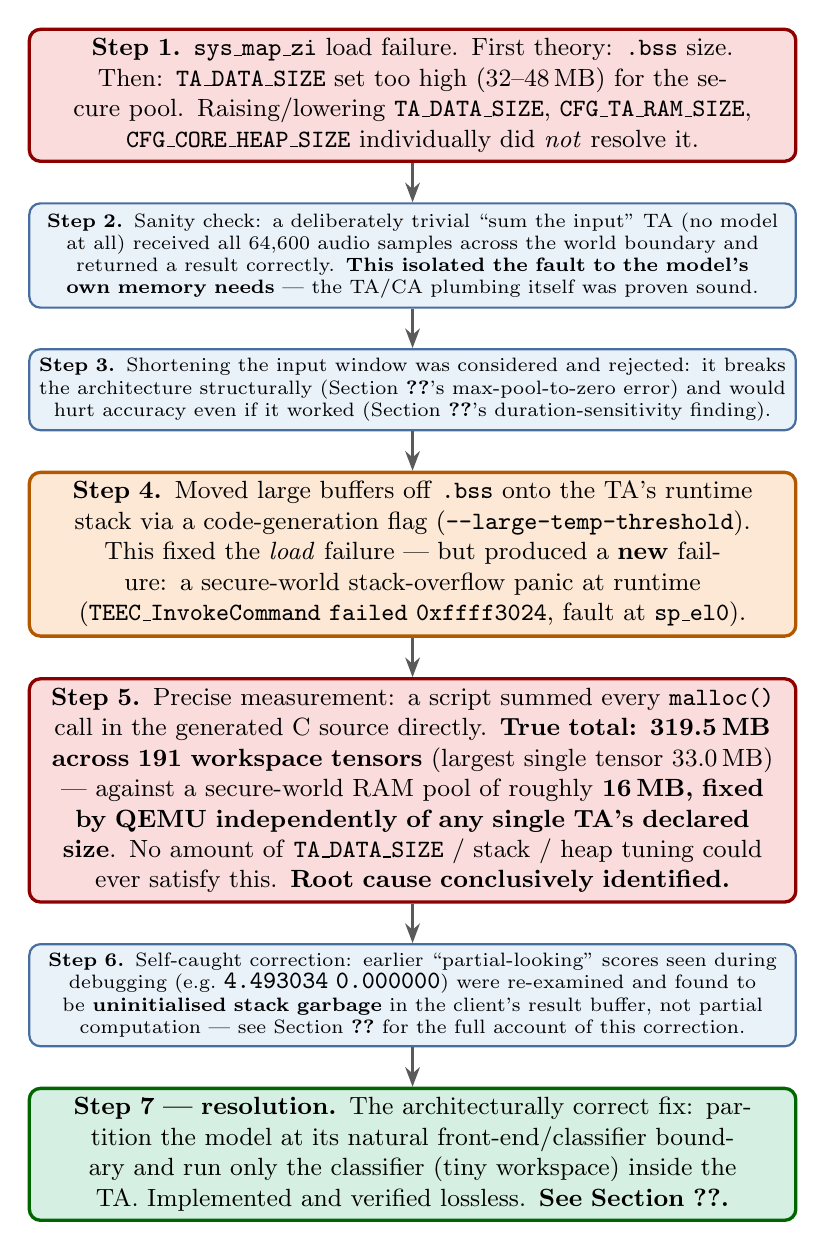
\begin{tikzpicture}[node distance=5mm]
\node[redblock, text width=9.5cm] (s1) {\textbf{Step 1.} \code{sys\_map\_zi} load failure.
First theory: \code{.bss} size. Then: \code{TA\_DATA\_SIZE} set too high (32--48\,MB) for the
secure pool. Raising/lowering \code{TA\_DATA\_SIZE}, \code{CFG\_TA\_RAM\_SIZE},
\code{CFG\_CORE\_HEAP\_SIZE} individually did \emph{not} resolve it.};
\node[smallblock, below=of s1, text width=9.5cm, fill=lightblue!70] (s2) {\textbf{Step 2.} Sanity
check: a deliberately trivial ``sum the input'' TA (no model at all) received all 64{,}600 audio
samples across the world boundary and returned a result correctly. \textbf{This isolated the fault
to the model's own memory needs} --- the TA/CA plumbing itself was proven sound.};
\node[smallblock, below=of s2, text width=9.5cm, fill=lightblue!70] (s3) {\textbf{Step 3.}
Shortening the input window was considered and rejected: it breaks the architecture structurally
(Section~\ref{sec:onnx2c-vs-emx}'s max-pool-to-zero error) and would hurt accuracy even if it
worked (Section~\ref{sec:rawtfnet}'s duration-sensitivity finding).};
\node[orangeblock, below=of s3, text width=9.5cm] (s4) {\textbf{Step 4.} Moved large buffers off
\code{.bss} onto the TA's runtime stack via a code-generation flag
(\code{--large-temp-threshold}). This fixed the \emph{load} failure --- but produced a
\textbf{new} failure: a secure-world stack-overflow panic at runtime
(\code{TEEC\_InvokeCommand failed 0xffff3024}, fault at \code{sp\_el0}).};
\node[redblock, below=of s4, text width=9.5cm] (s5) {\textbf{Step 5.} Precise measurement: a script
summed every \code{malloc()} call in the generated C source directly.
\textbf{True total: 319.5\,MB across 191 workspace tensors} (largest single tensor 33.0\,MB) ---
against a secure-world RAM pool of roughly \textbf{16\,MB, fixed by QEMU independently of any
single TA's declared size}. No amount of \code{TA\_DATA\_SIZE} / stack / heap tuning could ever
satisfy this. \textbf{Root cause conclusively identified.}};
\node[smallblock, below=of s5, text width=9.5cm, fill=lightblue!70] (s6) {\textbf{Step 6.}
Self-caught correction: earlier ``partial-looking'' scores seen during debugging (e.g.\
\code{4.493034 0.000000}) were re-examined and found to be \textbf{uninitialised stack garbage}
in the client's result buffer, not partial computation --- see Section~\ref{sec:garbage} for the
full account of this correction.};
\node[greenblock, below=of s6, text width=9.5cm] (s7) {\textbf{Step 7 --- resolution.} The
architecturally correct fix: partition the model at its natural
front-end/classifier boundary and run only the classifier (tiny workspace) inside the TA.
Implemented and verified lossless. \textbf{See Section~\ref{sec:partition}.}};
\draw[arrow] (s1) -- (s2);
\draw[arrow] (s2) -- (s3);
\draw[arrow] (s3) -- (s4);
\draw[arrow] (s4) -- (s5);
\draw[arrow] (s5) -- (s6);
\draw[arrow] (s6) -- (s7);
\end{tikzpicture}
\caption{Chronology of the memory-wall investigation, in the order it actually happened. Each step
either eliminated a hypothesis or narrowed the search, and the final measurement in Step 5 is what
turned an open-ended debugging problem into a conclusively settled root cause.}
\label{fig:memory-wall}
\end{figure}

\subsection{The self-caught misdiagnosis}
\label{sec:garbage}

\begin{crisisbox}{A mistake worth documenting honestly}
During Step 4's debugging, the TA occasionally returned scores such as \code{4.493034 0.000000} or
\code{6.403191 0.000000} instead of either a clean result or an outright failure. The first working
theory was that these represented \emph{partial computation} --- as if the model were somehow
tracking how far it got before running out of heap. \textbf{This theory was wrong}, and it was
caught and corrected before it could shape the eventual fix.
\end{crisisbox}

Reading the generated C source directly revealed the actual mechanism: \code{emx-onnx-cgen}'s
generated \code{model()} function allocates its $\sim$191 workspace tensors via a long sequence of
individual \code{malloc()} calls, and if \emph{any} of those calls fails, the function returns
silently \textbf{without writing to the output buffer at all}. The values that looked like ``partial
progress'' were simply whatever bytes happened to already be sitting in the client's uninitialised
\code{logits} array on the stack --- an artifact of C's lack of default zero-initialisation, not a
signal about the model. Once this was understood, the TA handler was changed to
zero-initialise \code{logits[2] = \{0.0f, 0.0f\}} before calling into the model, so that any future
silent allocation failure would show up as an unambiguous exact-zero result rather than a
plausible-looking but meaningless number. This fix is small, but the diagnostic discipline behind
it --- reading the generated source rather than trusting a superficially plausible pattern in the
output --- is what prevented a wrong root cause from being chased further.

\section{Phase 5 --- The fix: partitioning the model}
\label{sec:partition}

\begin{resolvedbox}{Resolution}
Rather than trying to fit a 319.5\,MB workspace into a $\sim$16\,MB secure-memory pool, the model
was split at its natural architectural seam --- the boundary between the front-end
(feature-extraction) stage and the classifier stage already visible in Figure~\ref{fig:rawtfnet-arch}
--- and only the small classifier half was compiled into the Trusted Application.
\end{resolvedbox}

This works because RawTFNet's own \code{forward()} method is already exactly
\code{classifier(front\_end(x))}: the split point already exists in the trained model's own
structure, so no retraining or architecture surgery was needed, only a different export boundary.

\begin{figure}[H]
\centering
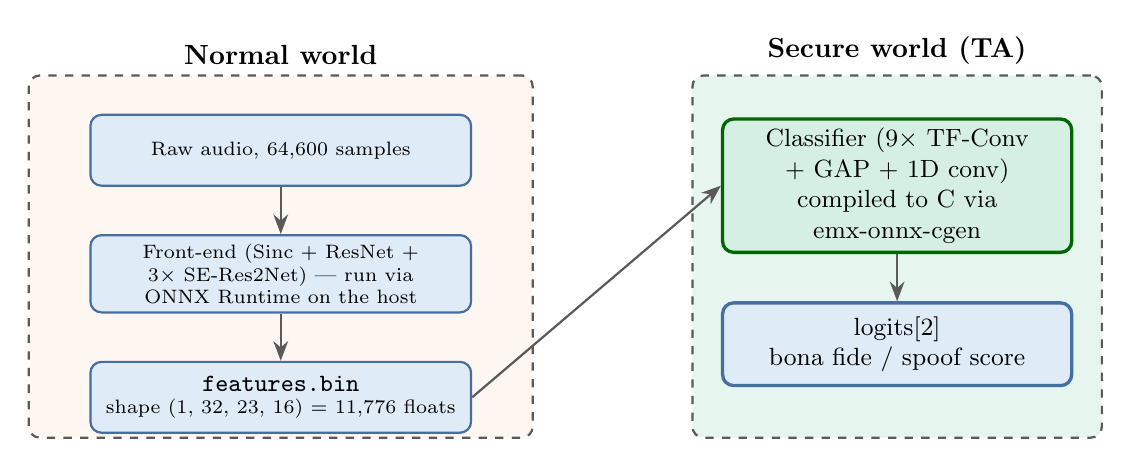
\begin{tikzpicture}[node distance=8mm and 14mm]
\node[worldbox, fill=peach!35, minimum width=6.4cm, minimum height=4.6cm] (nw) {};
\node[above] at (nw.north) {\textbf{Normal world}};
\node[worldbox, fill=mint!60, minimum width=5.2cm, minimum height=4.6cm, right=20mm of nw] (sw) {};
\node[above] at (sw.north) {\textbf{Secure world (TA)}};

\node[smallblock, text width=4.6cm] at ($(nw)+(0,1.35)$) (audio) {Raw audio, 64{,}600 samples};
\node[smallblock, text width=4.6cm, below=6mm of audio] (fe) {Front-end (Sinc + ResNet + 3$\times$
SE-Res2Net) --- run via ONNX Runtime on the host};
\node[smallblock, text width=4.6cm, below=6mm of fe] (feat) {\code{features.bin}\\ shape
(1, 32, 23, 16) = 11{,}776 floats};

\node[greenblock, text width=4.2cm] at ($(sw)+(0,0.9)$) (cls) {Classifier (9$\times$ TF-Conv +
GAP + 1D conv)\\ compiled to C via emx-onnx-cgen};
\node[block, text width=4.2cm, below=6mm of cls] (log) {logits[2]\\ bona fide / spoof score};

\draw[arrow] (audio) -- (fe);
\draw[arrow] (fe) -- (feat);
\draw[arrow] (feat.east) -- (cls.west);
\draw[arrow] (cls) -- (log);
\end{tikzpicture}
\caption{The partitioned deployment. The front-end runs unmodified in the normal world (feature
extraction is explicitly \emph{not} part of the confidentiality boundary for this PoC --- recorded
as a stated limitation in Chapter~\ref{ch:limitations}); only the classifier's forward pass, with
its far smaller workspace, executes inside the secure-world Trusted Application.}
\label{fig:partition}
\end{figure}

\subsection{Verifying the split is lossless}

Splitting a working model always raises one question: does the split itself introduce any error?
This was checked directly rather than assumed. \code{model.front\_end(x)} was run in PyTorch to
produce reference features, saved to \code{features.bin}; \code{model.classifier(features)} was run
separately and compared against the full model's single forward pass on the same input.

\begin{resolvedbox}{Verification result}
Classifier-only output matched the full-model forward pass \textbf{exactly}: \code{[[5.391142
$-$5.6215887]]} in both cases. The classifier's exported ONNX graph, compiled through
\code{emx-onnx-cgen}, then matched this reference at \textbf{7 ULP} maximum deviation. Final TA
configuration: \code{TA\_DATA\_SIZE} 4\,MB, \code{TA\_STACK\_SIZE} 256\,KB --- comfortably inside
the secure pool that the full model could never fit into. The TA loaded, ran, and returned
\textbf{\code{logits: 5.391142 -5.621588}} from inside the secure world, matching the PyTorch
reference to six decimal places.
\end{resolvedbox}

The pipeline was then verified on a \emph{second}, independent audio file
(\code{LA\_E\_1001928.flac}) to confirm this was not a one-off coincidence: PyTorch scored it
$-4.9850$; the secure-world TA scored the same file $-4.985014$ --- confirming the pipeline
generalises across inputs, not just the one file used during development.

\section{Phase 6 --- Any-audio pipeline and proof of secure-world execution}

With the partitioned model working, the pipeline was generalised to accept any user-supplied audio
file rather than a single fixed test vector, and then hardened for demonstration purposes.

\subsection{The any-audio pipeline}

A host-side script (\code{prepare\_audio.py}) loads an arbitrary \code{.wav}/\code{.flac} file via
\code{librosa} (which resamples to 16\,kHz automatically, resolving any sample-rate mismatch),
peak-normalises it, pads or repeats it to 64,600 samples, runs it through the exported front-end
ONNX graph, and writes the resulting features to a fixed shared-folder location that the QEMU guest
reads over a 9p virtio mount. The guest-side client application was changed to read this fixed path
automatically, so that a full round trip requires only \code{optee\_example\_rawtfnet} on the guest
side with no arguments, once the host-side preparation script has been run.

\subsection{Proving \emph{which} audio was processed, and that it happened in the secure world}

\begin{decisionbox}{Requirement raised during review}
It is not enough to show a correct-looking score; a reviewer needs independent evidence that (a)
the computation genuinely happened inside the secure world, and (b) it happened on the specific
audio file being claimed, not a stale or substituted result.
\end{decisionbox}

This was addressed by adding a second TA input parameter carrying the original filename as a label,
and logging it from \emph{inside} the secure world via \code{IMSG}: \code{=== SECURE WORLD:
processing audio file: <name> ===}, followed by a second \code{IMSG} line after inference with the
computed logits. Because this line is written to the Secure World console --- a log stream the
normal-world client application has no way to fabricate or edit --- it functions as independent,
tamper-resistant evidence of exactly which file was processed and that the processing occurred
inside TrustZone.

One build-configuration detail nearly hid this evidence entirely and is worth recording:
\code{ta/Makefile} sets \code{CFG\_TEE\_TA\_LOG\_LEVEL}, which defaults to \code{1} in the copied
example project. At that level, info-level \code{IMSG} output --- including both proof lines --- is
filtered out of the console, so the TA appeared to be running correctly while producing no visible
evidence at all. Raising the level to \code{3} made the proof lines appear as intended. This was
first discovered when a build that had aborted partway through (on the \code{cryptography}-module
error described below) left QEMU booting a \emph{stale} root filesystem image on the next run, so
the new logging code appeared not to be running even though the underlying TA logic was already
correct --- two separate causes stacked on top of each other, both resolved by (1)~ensuring the
full \code{make} completes without error before rebooting, and (2)~raising the log level.

\section{Phase 7 --- The domain-generalisation investigation}
\label{sec:ood}

\begin{crisisbox}{The finding}
Real-world audio --- Waleed's own recorded voice, an ElevenLabs text-to-speech spoof, and audio
supplied independently by the supervisor --- consistently misclassified as \textbf{SPOOF} through
the pipeline, including genuine bona fide recordings. The pipeline itself was working correctly
(verified repeatedly in Phases 5--6); this is a property of the \emph{model}, investigated as a
research question in its own right rather than treated as a bug to silently patch around.
\end{crisisbox}

This investigation proceeded as a controlled elimination study: each plausible cause was tested and
either fixed or ruled out, one at a time, before moving to the next.

\begin{figure}[H]
\centering
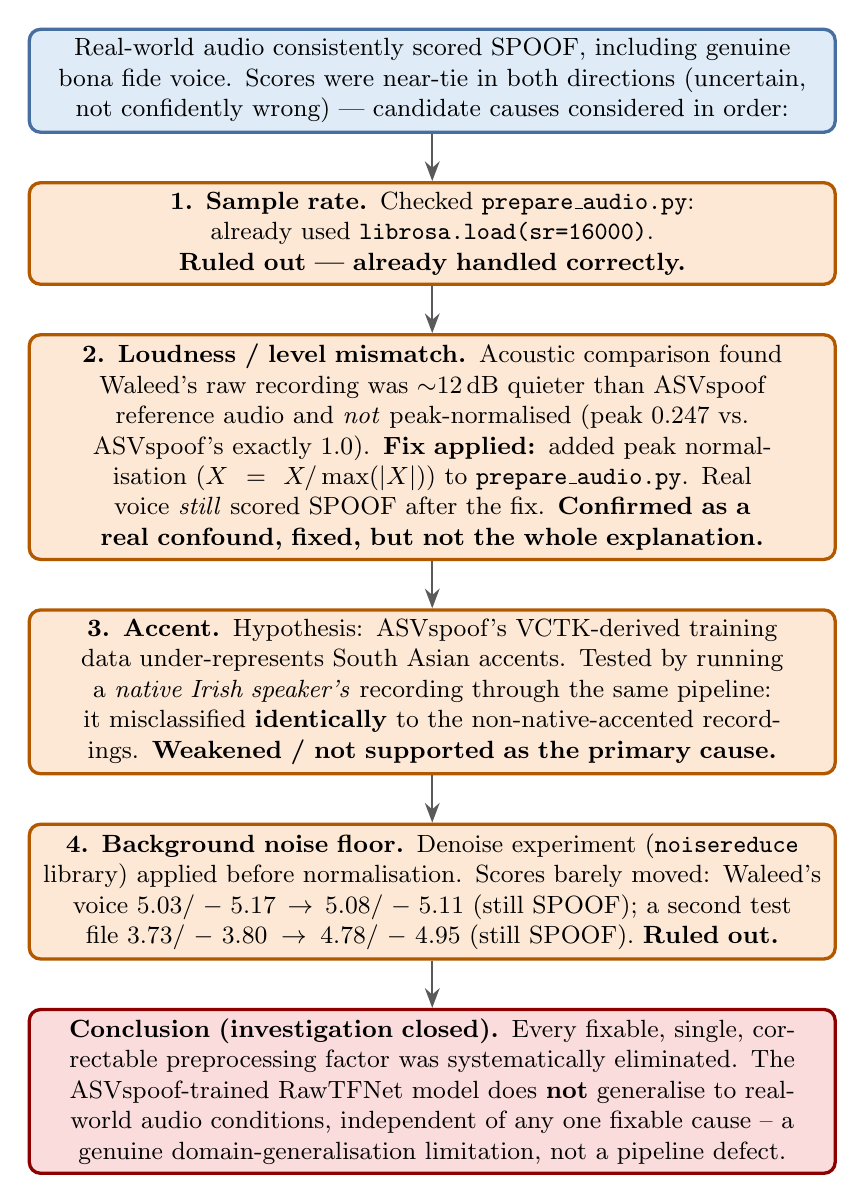
\begin{tikzpicture}[node distance=6mm]
\node[block, text width=10cm] (start) {Real-world audio consistently scored SPOOF, including
genuine bona fide voice. Scores were near-tie in both directions (uncertain, not confidently
wrong) --- candidate causes considered in order:};

\node[orangeblock, below=of start, text width=10cm] (c1) {\textbf{1. Sample rate.} Checked
\code{prepare\_audio.py}: already used \code{librosa.load(sr=16000)}. \textbf{Ruled out ---
already handled correctly.}};
\node[orangeblock, below=of c1, text width=10cm] (c2) {\textbf{2. Loudness / level mismatch.}
Acoustic comparison found Waleed's raw recording was $\sim$12\,dB quieter than ASVspoof reference
audio and \emph{not} peak-normalised (peak 0.247 vs.\ ASVspoof's exactly 1.0). \textbf{Fix applied:}
added peak normalisation ($X = X / \max(|X|)$) to \code{prepare\_audio.py}. Real voice \emph{still}
scored SPOOF after the fix. \textbf{Confirmed as a real confound, fixed, but not the whole
explanation.}};
\node[orangeblock, below=of c2, text width=10cm] (c3) {\textbf{3. Accent.} Hypothesis: ASVspoof's
VCTK-derived training data under-represents South Asian accents. Tested by running a
\emph{native Irish speaker's} recording through the same pipeline: it misclassified
\textbf{identically} to the non-native-accented recordings. \textbf{Weakened / not supported as
the primary cause.}};
\node[orangeblock, below=of c3, text width=10cm] (c4) {\textbf{4. Background noise floor.}
Denoise experiment (\code{noisereduce} library) applied before normalisation. Scores barely moved:
Waleed's voice $5.03/-5.17 \rightarrow 5.08/-5.11$ (still SPOOF); a second test file
$3.73/-3.80 \rightarrow 4.78/-4.95$ (still SPOOF). \textbf{Ruled out.}};
\node[redblock, below=of c4, text width=10cm] (concl) {\textbf{Conclusion (investigation closed).}
Every fixable, single, correctable preprocessing factor was systematically eliminated. The
ASVspoof-trained RawTFNet model does \textbf{not} generalise to real-world audio conditions,
independent of any one fixable cause -- a genuine domain-generalisation limitation, not a pipeline
defect.};
\draw[arrow] (start) -- (c1);
\draw[arrow] (c1) -- (c2);
\draw[arrow] (c2) -- (c3);
\draw[arrow] (c3) -- (c4);
\draw[arrow] (c4) -- (concl);
\end{tikzpicture}
\caption{The out-of-distribution elimination study: each candidate cause of real-world
misclassification was tested individually before being ruled in, ruled out, or fixed. Sample rate
was already correct; loudness was a real, fixable confound that was fixed but did not resolve the
misclassification; accent was weakened as an explanation by a same-pipeline native-speaker control;
noise floor was ruled out directly. What remains is attributed to the trained model keying on
dataset-specific synthesis artefacts of ASVspoof rather than general spoof characteristics.}
\label{fig:ood}
\end{figure}

\begin{findingbox}{A refinement, not a reversal}
Audio clips later supplied independently by the supervisor (Dr.\ Foley) as an out-of-sample speaker
test refined rather than overturned this conclusion. One clip (\code{Rec 1.flac}) scored bona fide
$0.54$ vs.\ spoof $-0.74$ --- still classified SPOOF (incorrect, it was a genuine recording), but
with scores an order of magnitude closer to the decision boundary than every prior real-world file,
which had scored confidently in the 3--5 range. This suggests the domain gap is better described as
a \textbf{spectrum} than a wall: the degree of misclassification varies by recording, and this
particular clip landed almost exactly on the fence. The remaining four supplied clips
(\code{Rec 2--5.flac}) are queued to run through the same pipeline as a next step.
\end{findingbox}

\subsection{Why this is framed as a finding, not a failure}

Framed correctly, this investigation is legitimate thesis content, not a setback to hide. The
confidential-inference gateway itself --- the actual subject of this proof-of-concept --- works
flawlessly, proven end-to-end with independent secure-world evidence (Phase 6). The
detector's real-world accuracy is a separate, now rigorously characterised research problem, with a
clear recommended path forward: report batch accuracy/EER on in-distribution ASVspoof evaluation
data, present this elimination study as a results/limitations chapter, and name domain adaptation
or fine-tuning on real-world and TTS audio as explicit future work. This mirrors exactly the
generalisation gap that the project's own literature review identifies as an open problem across the
field (Chapter~\ref{sec:rq}, RQ1), which places this project's own empirical finding in direct
conversation with the surrounding literature rather than as an isolated anecdote.

\section{Phase 8 --- Live Asterisk call integration}
\label{sec:asterisk}

The final phase of the work in progress at the time of writing is wiring the verified secure-world
pipeline to a live phone call, so that a verdict streams during the call rather than after it ends.

\subsection{Design: sliding window, not record-then-analyse}

\begin{figure}[H]
\centering
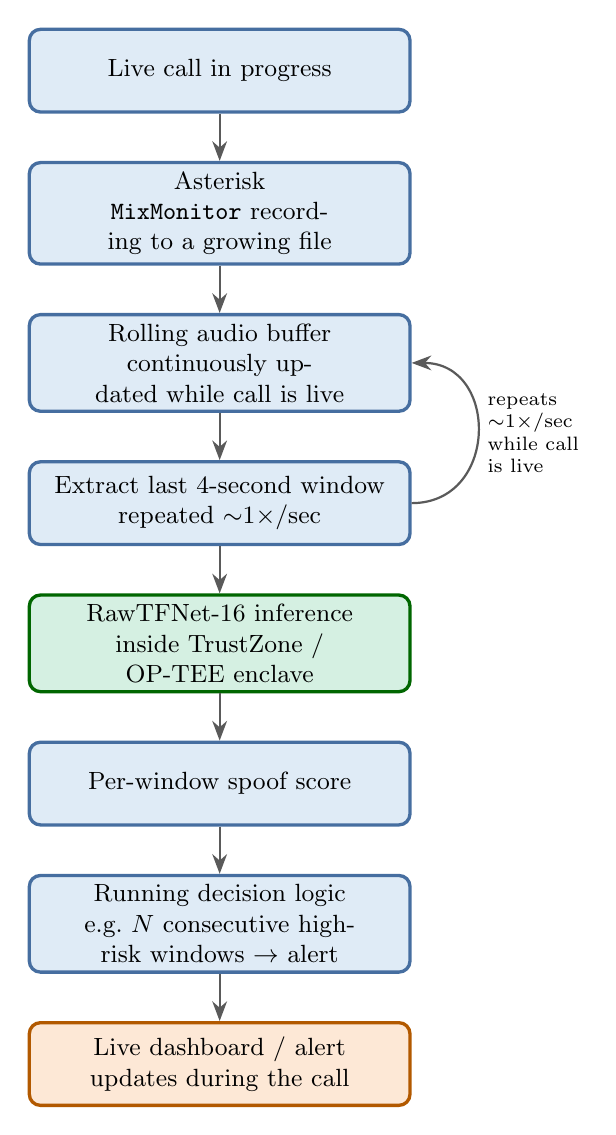
\begin{tikzpicture}[node distance=6mm]
\node[block] (call) {Live call in progress};
\node[block, below=of call] (ast) {Asterisk\\ \code{MixMonitor} recording to a growing file};
\node[block, below=of ast] (buf) {Rolling audio buffer\\ continuously updated while call is live};
\node[block, below=of buf] (win) {Extract last 4-second window\\ repeated $\sim$1$\times$/sec};
\node[greenblock, below=of win] (inf) {RawTFNet-16 inference\\ inside TrustZone / OP-TEE enclave};
\node[block, below=of inf] (sc) {Per-window spoof score};
\node[block, below=of sc] (dec) {Running decision logic\\ e.g.\ $N$ consecutive high-risk windows
$\rightarrow$ alert};
\node[orangeblock, below=of dec] (dash) {Live dashboard / alert\\ updates during the call};
\draw[arrow] (call) -- (ast);
\draw[arrow] (ast) -- (buf);
\draw[arrow] (buf) -- (win);
\draw[arrow] (win) -- (inf);
\draw[arrow] (inf) -- (sc);
\draw[arrow] (sc) -- (dec);
\draw[arrow] (dec) -- (dash);
\draw[arrow] (win.east) to [out=0,in=0,looseness=1.6] node[right, font=\scriptsize, align=left]
{repeats\\ $\sim$1$\times$/sec\\ while call\\ is live} (buf.east);
\end{tikzpicture}
\caption{Live in-call sliding-window design. A single noisy window is prevented from triggering a
false alarm mid-call by requiring several consecutive high-risk windows before an alert is raised,
the same overlapping-chunk pattern used by live captioning or live translation systems.}
\label{fig:sliding-window}
\end{figure}

The 4-second window length is not arbitrary: it matches RawTFNet's own training segment length and
the duration-sensitivity finding recorded in Section~\ref{sec:rawtfnet} (accuracy is worst on clips
under 2 seconds). Shortening the window to reduce latency was considered and rejected for exactly
this reason.

\subsection{What this requires from Asterisk, and what was actually built for this PoC}

A genuinely live pipeline would stream audio out of Asterisk while the call is still connected
(via AudioSocket or the Asterisk REST Interface with external media) into a long-running detection
service. For this proof-of-concept phase, a pragmatic intermediate step was built instead: Asterisk
was installed on the Ubuntu VM with a SIP endpoint and a dialplan extension that answers a call and
records it continuously via \code{MixMonitor} to a growing file; a host-side watcher script
(\code{live\_detect.py}) polls that growing recording, and every 4 seconds extracts the newest
64,600-sample window, peak-normalises it, runs it through the front-end, and signals the QEMU guest
to run a fresh secure-world inference --- reproducing the sliding-window behaviour of
Figure~\ref{fig:sliding-window} against a call that is still being recorded, ahead of migrating to a
true streaming capture method.

\begin{resolvedbox}{Status at time of writing}
Asterisk installation, SIP endpoint (\code{100}) and dialplan (extension \code{600}) configuration,
and MicroSIP softphone registration are complete and confirmed working: a test call was placed and
the recording file (\code{/tmp/live.wav16}) was observed growing in real time during the call. The
full end-to-end demonstration --- watcher loop plus \code{live\_detect.py} plus a live call
producing a stream of secure-world verdicts --- has been re-explained in full and is the next
concrete milestone, not yet reported as executed end-to-end at the time of writing.
\end{resolvedbox}

\chapter{Verification Summary}

Table~\ref{tab:verification} consolidates every point in the pipeline where a numerical or
behavioural claim was independently checked, rather than assumed, because this is the evidence base
the thesis's correctness claims ultimately rest on.

\begin{table}[H]
\centering
\small
\begin{tabularx}{\textwidth}{@{}p{3.6cm}X@{}}
\toprule
\textbf{Checkpoint} & \textbf{Evidence} \\
\midrule
OP-TEE environment & \code{xtest}: 0 failures across 41{,}482 subtests, 145 test cases \\
TA/CA communication pattern & \code{hello\_world} round trip: value 42 correctly incremented to 43
across the secure-world boundary \\
PyTorch $\to$ ONNX export & Scores match to four decimal places on a held-out ASVspoof utterance
(PyTorch $-5.6216$, ONNX $-5.6216$) \\
ONNX $\to$ TVM (independent cross-check) & TVM/Relax output $-5.621588$, matching both prior stages
\\
ONNX $\to$ C (emx-onnx-cgen) & Built-in \code{verify} against ONNX Runtime: max deviation 7 ULP \\
Front-end / classifier split & Classifier-only output identical to full-model forward pass:
\code{5.391142, $-$5.6215887} in both cases \\
In-TA classifier execution & Secure-world TA returned \code{5.391142 -5.621588}, matching the
PyTorch reference to six decimal places \\
Generalisation to a second file & PyTorch $-4.9850$ vs.\ secure-world $-4.985014$ on an independent
test file (\code{LA\_E\_1001928.flac}) \\
Secure-world execution proof & \code{IMSG} filename + score logged from inside the secure world,
independently visible on a console the normal-world CA cannot write to \\
\bottomrule
\end{tabularx}
\caption{Every correctness or behavioural claim in this document that was independently verified,
with the evidence produced at each stage.}
\label{tab:verification}
\end{table}

\chapter{Limitations and Threats to Validity}
\label{ch:limitations}

These are stated explicitly here, in the same form intended for the thesis's own Limitations
section, so that nothing in this document overstates what has actually been demonstrated.

\begin{table}[H]
\centering
\small
\begin{tabularx}{\textwidth}{@{}p{3.9cm}X@{}}
\toprule
\textbf{Limitation} & \textbf{Explanation} \\
\midrule
No physical target hardware & All results were obtained on the QEMU ARMv8-A \code{virt} reference
platform, not a physical Raspberry Pi 4. This validates the software architecture and the
TrustZone isolation model, not device-specific behaviour (boot chain, peripheral timing, thermal
characteristics of the BCM2711 SoC). \\
No hardware root of trust & QEMU's secure world is a software CPU-mode partition: no fused keys,
no physical secure boot chain, no tamper resistance. Hardware-backed attestation is out of scope
and identified as future work. \\
Static, compiled-in model weights & The PoC keeps model weights as a static array compiled
directly into the TA binary, skipping secure storage / key-provisioning. Not workable for the
longer-term federated-learning goal, but a reasonable simplification for a feasibility PoC. \\
Feature extraction stays in the normal world & Only the classifier's forward pass runs inside the
secure world; audio windowing and front-end feature extraction remain in the untrusted normal
world. This is a deliberate, stated scope boundary, not an oversight --- an attacker with
normal-world root could in principle feed the TA manipulated features. \\
Emulation performance is not representative & QEMU/TCG software translation is expected to be one
to two orders of magnitude slower than native Pi 4 execution for this workload. Any latency claims
from this phase must be reported explicitly as QEMU-only figures. \\
Real-world detection accuracy & Systematically characterised in Section~\ref{sec:ood}: the
ASVspoof-trained model does not reliably generalise to real-world recording conditions. This is
reported as a research finding with a defined future-work path (domain adaptation / fine-tuning),
not hidden or worked around. \\
Live capture is not yet streaming & The Asterisk integration currently polls a growing
\code{MixMonitor} recording rather than receiving a true live audio stream (AudioSocket / ARI
external media); this is the next milestone. \\
Toolchain instability & Apache TVM 0.25.0.post1's Relax API differs enough from most published
tutorials that import paths had to be resolved empirically; pinning a specific, documented TVM
version is recommended before final submission. \\
Timing / side-channel hardening out of scope & No side-channel hardening (cache-timing, power
analysis) has been attempted. Reasonable to state explicitly as future work rather than an
oversight. \\
\bottomrule
\end{tabularx}
\caption{Consolidated limitations and threats to validity.}
\label{tab:limitations}
\end{table}

\chapter{Positioning Against the Literature Review}
\label{sec:rq}

The project's literature review is organised around three research questions; this proof-of-concept
speaks most directly to the second, and its own empirical findings connect back to the first.

\begin{table}[H]
\centering
\small
\begin{tabularx}{\textwidth}{@{}p{1.6cm}X@{}}
\toprule
\textbf{RQ} & \textbf{How this PoC relates} \\
\midrule
RQ1 & Which post-2020 detection architectures best balance EER against edge computational
footprint? RawTFNet-16 was selected precisely on this basis (Table~\ref{tab:rawtfnet-compare}).
This project's own out-of-distribution elimination study (Section~\ref{sec:ood}) is direct,
first-hand evidence for the review's finding that accuracy drops sharply once audio moves from
clean academic datasets to real-world conditions. \\
RQ2 & How can federated learning, differential privacy, and TrustZone-based confidential inference
be combined for end-to-end privacy guarantees? No peer-reviewed study combines all three
specifically for anti-spoofing; the literature review treats their combination as a proposed
synthesis rather than something already validated. \textbf{This PoC is the first concrete,
working piece of that synthesis} --- it demonstrates that the TrustZone/confidential-inference
primitive alone is achievable end-to-end with a real anti-spoofing model, which is the load-bearing
precondition for layering federated learning and differential privacy on top in subsequent work. \\
RQ3 & What deployment challenges remain in moving detection from lab benchmarks to the residential
telephony edge? The Asterisk integration work (Section~\ref{sec:asterisk}) is a direct, concrete
attempt at exactly this transfer, and the domain-generalisation finding is first-hand evidence of
the widening lab-to-real-world performance gap the review identifies as a field-wide open problem.
\\
\bottomrule
\end{tabularx}
\caption{How this proof-of-concept's work maps onto the thesis's three research questions.}
\label{tab:rq}
\end{table}

\chapter{Current Status and Next Steps}

\section{Where the project stands}

\begin{itemize}[leftmargin=1.4em]
  \item The confidential-inference core is \textbf{complete and verified end-to-end}: a
  partitioned RawTFNet-16 classifier runs inside an OP-TEE Trusted Application on QEMU, produces
  scores matching the original PyTorch model to six decimal places, and provides independent
  secure-world evidence of which audio file it processed.
  \item The any-audio pipeline is working and has been demonstrated on multiple files, including
  ASVspoof evaluation clips (correct classification) and real-world recordings (the characterised
  domain-generalisation limitation of Section~\ref{sec:ood}).
  \item Asterisk is installed, configured, and confirmed capturing live call audio; the watcher-loop
  integration with the secure-world pipeline has been designed and documented but not yet reported
  as run end-to-end.
\end{itemize}

\section{Immediate next steps}

\begin{enumerate}[leftmargin=1.5em]
  \item Run the remaining supervisor-supplied clips (\code{Rec 2--5.flac}) through the pipeline to
  extend the near-boundary observation from \code{Rec 1.flac} into a small independent-speaker
  result set.
  \item Complete and report the first full end-to-end live-call demonstration: watcher loop,
  \code{live\_detect.py}, and a live call producing a visible stream of secure-world verdicts.
  \item Produce a batch accuracy / EER measurement across a larger sample of ASVspoof evaluation
  files (20--50 files), to report a proper in-distribution accuracy figure alongside the
  out-of-distribution findings.
  \item Add TA-side timing instrumentation to capture clean QEMU inference-latency numbers, explicitly
  labelled as non-representative of Pi 4 performance per Section~\ref{sec:qemu-vs-pi4}, as a
  baseline for later comparison if physical Pi 4 hardware becomes available.
  \item Migrate the live-call capture path from polling a growing \code{MixMonitor} recording to a
  genuine streaming source (AudioSocket or ARI external media), closing the last gap identified in
  Table~\ref{tab:limitations}.
\end{enumerate}

\chapter{Summary}

The confidential-inference phase of this thesis set out to answer one question: can a trained
audio-deepfake detector be made to run inside an ARM TrustZone secure world, with its correctness
provable end-to-end, on hardware actually available during this phase of the project? The answer,
demonstrated and verified repeatedly rather than assumed, is yes --- but the path there was not
straightforward, and this document has tried to be honest about that rather than presenting only the
final working state.

Three points are worth restating together, because they are the ones a supervisor is most likely to
probe: first, every substitution made along the way --- QEMU for a physical Pi 4, a VM for WSL2, ONNX
compilation for hand-ported C --- was a deliberate, justified engineering decision with a stated
cost, not an unexamined convenience. Second, the memory-wall failure in
Section~\ref{sec:memory-wall} was a genuine, multi-day obstacle that was resolved by measurement
and architectural redesign (partitioning the model at its natural seam) rather than by parameter
tuning, and the self-caught misdiagnosis along the way is included deliberately, as evidence of the
diagnostic process rather than something to omit. Third, the real-world misclassification finding in
Section~\ref{sec:ood} was investigated with the same rigour as any other result in this document ---
systematically, one variable at a time --- and the conclusion that emerged is a legitimate research
contribution about the limits of the ASVspoof-trained model, directly connected to a gap the
thesis's own literature review already identifies as open in the field.

The confidential-inference gateway --- the actual subject of this proof-of-concept --- works. What
remains is extending it to a fully streaming live-call demonstration, and reporting the detector's
accuracy honestly across both the conditions it was trained for and the conditions it was not.

\end{document}
